%%%%%%%%%%%%  Generated using docx2latex.com  %%%%%%%%%%%%%%

%%%%%%%%%%%%  v2.0.0-beta  %%%%%%%%%%%%%%

\documentclass[12pt]{book}

\usepackage{amsmath}
\usepackage{latexsym}
\usepackage{amsfonts}
\usepackage[normalem]{ulem}
\usepackage{soul}
\usepackage{array}
\usepackage{amssymb}
\usepackage{extarrows}
\usepackage{graphicx}
%\usepackage[backend=biber,
%style=numeric,
%sorting=none,
%isbn=false,
%doi=false,
%url=false,
%]{biblatex}\addbibresource{bibliography.bib}

\usepackage{subfig}
\usepackage{wrapfig}
\usepackage{txfonts}
\usepackage{wasysym}
\usepackage{enumitem}
\usepackage{adjustbox}
\usepackage{ragged2e}
\usepackage[svgnames,table]{xcolor}
\usepackage{tikz}
\usepackage{longtable}
%\usepackage{changepage}
\usepackage{setspace}
\usepackage{hhline}
\usepackage{multicol}
\usepackage{tabto}
\usepackage{float}
\usepackage{multirow}
\usepackage{makecell}
\usepackage{fancyhdr}
\usepackage[toc,page]{appendix}
\usepackage[hidelinks]{hyperref}
\usetikzlibrary{shapes.symbols,shapes.geometric,shadows,arrows.meta}
\tikzset{>={Latex[width=1.5mm,length=2mm]}}
\usepackage{flowchart}
\usepackage[
paperheight=29.7 cm,
paperwidth=21 cm,
left=1.25in,
right=1.25in,
top=1.0in,
bottom=1.0in,
headheight=1in]{geometry}
\usepackage[utf8]{inputenc}
\usepackage[T1]{fontenc}
\TabPositions{0.5in,1.0in,1.5in,2.0in,2.5in,3.0in,3.5in,4.0in,4.5in,5.0in,5.5in,}
\usepackage{mathptmx}% Times Roman font
\urlstyle{same}

\usepackage[croatian]{babel}
\usepackage{setspace}
\usepackage{lipsum}
\usepackage{multirow}
\makeatletter
\setlength{\@fptop}{0 pt}
\makeatother
\graphicspath{{Slike/}}

\renewcommand{\thefootnote}{\fnsymbol{footnote}}


 %%%%%%%%%%%% Literatura  %%%%%%%%%%%%%%
\usepackage[square,numbers,sort]{natbib}

%\pgfplotsset{
%	legend entry/.initial=,
%	every axis plot post/.code={%
%		\pgfkeysgetvalue{/pgfplots/legend entry}\tempValue
%		\ifx\tempValue\empty
%		\pgfkeysalso{/pgfplots/forget plot}%
%		\else
%		\expandafter\addlegendentry\expandafter{\tempValue}%
%		\fi
%	},
%}


 %%%%%%%%%%%%  Set Depths for Sections  %%%%%%%%%%%%%%

% 1) Section
% 1.1) SubSection
% 1.1.1) SubSubSection
% 1.1.1.1) Paragraph
% 1.1.1.1.1) Subparagraph


\setcounter{tocdepth}{5}
\setcounter{secnumdepth}{5}


 %%%%%%%%%%%%  Set Depths for Nested Lists created by \begin{enumerate}  %%%%%%%%%%%%%%


\setlistdepth{9}
\renewlist{enumerate}{enumerate}{9}
		\setlist[enumerate,1]{label=\arabic*)}
		\setlist[enumerate,2]{label=\alph*)}
		\setlist[enumerate,3]{label=(\roman*)}
		\setlist[enumerate,4]{label=(\arabic*)}
		\setlist[enumerate,5]{label=(\Alph*)}
		\setlist[enumerate,6]{label=(\Roman*)}
		\setlist[enumerate,7]{label=\arabic*}
		\setlist[enumerate,8]{label=\alph*}
		\setlist[enumerate,9]{label=\roman*}

\renewlist{itemize}{itemize}{9}
		\setlist[itemize]{label=$\cdot$}
		\setlist[itemize,1]{label={--}}
		\setlist[itemize,2]{label=$\circ$}
		\setlist[itemize,3]{label=$\ast$}
		\setlist[itemize,4]{label=$\dagger$}
		\setlist[itemize,5]{label=$\triangleright$}
		\setlist[itemize,6]{label=$\bigstar$}
		\setlist[itemize,7]{label=$\blacklozenge$}
		\setlist[itemize,8]{label=$\prime$}



 %%%%%%%%%%%%  Header here  %%%%%%%%%%%%%%


\pagestyle{fancy}
\fancyhf{}
%\cfoot{ 
%\vspace{\baselineskip}
%}
\fancyfoot[R]{\thepage}
%\fancyfoot[L]{\thepage}
\renewcommand{\headrulewidth}{0pt}
\setlength{\topsep}{0pt}\setlength{\parindent}{0pt}
\renewcommand{\arraystretch}{1.3}

%%%%%%%%%%%%%%%%%	Naslovi bez aoisd	%%%%%%%%%%%%%%%%%%%%%%%%%%%

\makeatletter
\def\@makechapterhead#1{%
	\vspace*{50\p@}%
	{\parindent \z@ \raggedright \normalfont
		\ifnum \c@secnumdepth >\m@ne
		\if@mainmatter
		\Huge\bfseries \thechapter.\space%
		%\par\nobreak
		%\vskip 20\p@
		\fi
		%
		\Huge \bfseries \uppercase{#1}\par\nobreak
		\vskip 40\p@
		
	
}}
\makeatother





\usepackage{titlesec}



%%%%%%%%%%%%%%%%%%%% Document code starts here %%%%%%%%%%%%%%%%%%%%

\newcommand{\autor} {Fredrik Lamb}
\newcommand{\studij} {Preddiplomski sveučilišni}
\newcommand{\smjer} {Pozitivan}
\newcommand{\kolegij} {Filozofija građevinarstva}
\newcommand{\naslov}{Tko pije, a tko plaća na neaktivnom gradilištu?}
\newcommand{\JMBAG} {000111222}
\newcommand{\vrsta}{Završni rad} % ili Diplomski





%%



\onehalfspacing

\begin{document}

\thispagestyle{empty}

\vspace{\baselineskip}
\begin{Center}
{\fontsize{14pt}{16.8pt}\selectfont \textbf{SVEUČILIŠTE U RIJECI}\par}
\end{Center}\par

\begin{Center}
{\fontsize{14pt}{16.8pt}\selectfont \textbf{GRAĐEVINSKI FAKULTET}\par}
\end{Center}\par


\vspace{\baselineskip}
\begin{Center}
{\fontsize{14pt}{16.8pt}\selectfont \textbf{Prijediplomski Sveučilišni studij}\par}
\end{Center}\par

\begin{Center}
{\fontsize{14pt}{16.8pt}\selectfont \textbf{Građevinarstvo}\par}
\end{Center}\par

\begin{Center}
{\fontsize{14pt}{16.8pt}\selectfont \textbf{ {Mehanika II} }\par}
\end{Center}\par


%\vspace{\baselineskip}
%
%\vspace{\baselineskip}
%
%\vspace{\baselineskip}
%
%\vspace{\baselineskip}
%
%%\vspace{\baselineskip}
%
%%\vspace{\baselineskip}
%
%\vspace{\baselineskip}
%
%\vspace{\baselineskip}
%
%\vspace{\baselineskip}
%
%\vspace{\baselineskip}
%
%\vspace{\baselineskip}
%
%\vspace{\baselineskip}

\vskip 144pt

\begin{Center}
{\fontsize{14pt}{16.8pt}\selectfont \textbf{Lovro Korpar}\par}
\end{Center}\par

\begin{Center}
{\fontsize{14pt}{16.8pt}\selectfont \textbf{0114035332}\par}
\end{Center}\par


\vspace{\baselineskip}

\vspace{\baselineskip}

\vspace{\baselineskip}
\begin{Center}
{\fontsize{14pt}{16.8pt}\selectfont \textbf{ {Utjecaj promjene mase i širine ploče jednokatnog modela na dinamički odgovor na pobudu podloge} }\par}
\end{Center}\par


\vspace{\baselineskip}

\vspace{\baselineskip}

\vspace{\baselineskip}
\begin{Center}
\textbf{{\vrsta}}
\end{Center}\par


\vspace{\baselineskip}

\vspace{\baselineskip}

\vspace{\baselineskip}

\vspace{\baselineskip}

\vspace{\baselineskip}

\vspace{\baselineskip}

\vspace{\baselineskip}

\vspace{\baselineskip}

\vspace{\baselineskip}
\begin{Center}
\textbf{Rijeka, {\today}}
\end{Center}\par

\thispagestyle{empty}

\vspace{\baselineskip}
\begin{Center}
	{\fontsize{14pt}{16.8pt}\selectfont \textbf{SVEUČILIŠTE U RIJECI}\par}
\end{Center}\par

\begin{Center}
	{\fontsize{14pt}{16.8pt}\selectfont \textbf{GRAĐEVINSKI FAKULTET}\par}
\end{Center}\par


\vspace{\baselineskip}
\begin{Center}
	{\fontsize{14pt}{16.8pt}\selectfont \textbf{Prijediplomski Sveučilišni studij}\par}
\end{Center}\par

\begin{Center}
	{\fontsize{14pt}{16.8pt}\selectfont \textbf{Građevinarstvo}\par}
\end{Center}\par

\begin{Center}
	{\fontsize{14pt}{16.8pt}\selectfont \textbf{ {Mehanika II} }\par}
\end{Center}\par


%\vspace{\baselineskip}
%
%\vspace{\baselineskip}
%
%\vspace{\baselineskip}
%
%\vspace{\baselineskip}
%
%%\vspace{\baselineskip}
%
%%\vspace{\baselineskip}
%
%\vspace{\baselineskip}
%
%\vspace{\baselineskip}
%
%\vspace{\baselineskip}
%
%\vspace{\baselineskip}
%
%\vspace{\baselineskip}
%
%\vspace{\baselineskip}

\vskip 144pt

\begin{Center}
	{\fontsize{14pt}{16.8pt}\selectfont \textbf{Lovro Korpar}\par}
\end{Center}\par

\begin{Center}
	{\fontsize{14pt}{16.8pt}\selectfont \textbf{0114035332}\par}
\end{Center}\par


\vspace{\baselineskip}

\vspace{\baselineskip}

\vspace{\baselineskip}
\begin{Center}
	{\fontsize{14pt}{16.8pt}\selectfont \textbf{ {Utjecaj promjene mase i širine ploče jednokatnog modela na dinamički odgovor na pobudu podloge} }\par}
\end{Center}\par


\vspace{\baselineskip}

\vspace{\baselineskip}

\vspace{\baselineskip}
\begin{Center}
	\textbf{{\vrsta}}
\end{Center}\par


\vspace{\baselineskip}

\vspace{\baselineskip}

\vspace{\baselineskip}

\vspace{\baselineskip}

\vspace{\baselineskip}

\vspace{\baselineskip}

\vspace{\baselineskip}

\vspace{\baselineskip}

\vspace{\baselineskip}
\begin{Center}
	\textbf{Rijeka, {\today}}
\end{Center}\par

%\begin{justify}


 %%%%%%%%%%%%  Starting New Page here %%%%%%%%%%%%%%

\newpage

\thispagestyle{empty}
\mbox{}
\thispagestyle{empty}

\newpage

\thispagestyle{empty}
\mbox{}
\thispagestyle{empty}


\vskip 48 pt

\begin{center}
{\fontsize{14pt}{16.8pt}\selectfont \textbf{IZJAVA}\par}\par
\end{center}\par

\vspace{\baselineskip}

\vspace{\baselineskip}
\begin{justify}
	\begin{onehalfspace}
Završni rad izradio sam samostalno, u suradnji s mentoricom i uz poštivanje pozitivnih građevinskih propisa i znanstvenih dostignuća iz područja građevinarstva. Građevinski fakultet u Rijeci je nositelj prava intelektualnog vlasništva u odnosu na ovaj rad. 
	\end{onehalfspace}

\end{justify}\par


\vspace{\baselineskip}

\vspace{\baselineskip}

\vspace{\baselineskip}
\_\_\_\_\_\_\_\_\_\_\_\_\_\_\_\_\_\_\_\_\_\_\_\_\_\_\_\_\_\_\_\_\_\_\_\_\_\_\_\_\_\_ \par

{Lovro Korpar}\par



\vskip 60 pt
U Rijeci, {\today}\par

\newpage

\thispagestyle{empty}
\mbox{}
\thispagestyle{empty}

\pagestyle{empty}
\begin{center}
	\textbf{ZAHVALA}
\end{center}

Zahvaljujem se mentorici dr.sc. Nini Čeh na mentorstvu, uloženom trudu, dobroj volji, te pomoći oko izrade završnog rada. Također zahvaljujem se na dodatnom znanju kojeg sam stekao tokom izrade ovog završnog rada, te mogućnosti rada u laboratoriju.

Zahvaljujem se svojoj obitelji, posebno mom pokojnom ocu bez čijih priča nebi upisao ovaj fakultet, te majci na najvećoj podršci koju čovjek može dobiti.


\cleardoublepage
\begin{flushleft}
	
\end{flushleft}

\pagenumbering{roman}
\setcounter{page}{1}

\tableofcontents
\cleardoublepage

\addcontentsline{toc}{chapter}{\listfigurename}\listoffigures

\cleardoublepage
\addcontentsline{toc}{chapter}{\listtablename}\listoftables


\clearpage

\pagenumbering{arabic}
\pagestyle{plain}
\setcounter{page}{1}

\chapter{Uvod}
Potres je iznenadna prirodna pojava kratkotrajnih vibracija površine Zemlje. Izazvana je spontanim i naglim oslobađanjem energije uslijed pokreta pojedinih dijelova Zemljine kore duž rasjeda. Istraživanjem potresa, odnosno seizmičkih valova bavi se geofizička disciplina seizmologija. Danas poznajemo razne vrste potresa, ali kao glavnim i najučestalijim potresima smatramo one koji su nastali kao posljedica tektonskih poremećaja koji izazivaju pucanje i vibracije na površini Zemlje kao i na objektima. Uzimajući u obzir ove stvari od građevinara se očekuje da objekte koje izgrade budu otporni na pobudu potresa i da utjecaj potresa na objekte bude minimalan. Za istraživanje novih solucija koje bi pomogle u tome, provode se laboratorijska ispitivanja. U laboratorijskim ispitivanjima koriste se posebni modeli koji imitiraju konstrukciju pri pobudi potresa. 

U ovom završnom radu će se promatrati kako promjena dimenzija konstukcije, te samim time i promjena mase utječe na pobudu potresa.

\chapter{Potresi i njihovi utjecaj na gra\DJ evine}
Zemlja se povremeno potresa u obliku brzo izmjenjenih vibracija litosfere koje uzrokuju valovi koji prenose energiju u svim smjerovima iz nekog podzemnog žarišta (epicentra). Potrese, njihova žarišta, smjerove, vrijeme trajanja i jačinu ne možemo predvidjeti. Ali kao pomoć razumijevanju potresa služe nam seizmološke stanice na kojima se svake godine zabilježi preko 1 milijun potresa diljem svijeta. Svi zabilježeni potresi su nam bitni, ali najbitniji su nam oni u naseljenim područjima. Kod potresa u naseljenim područjima možemo vidjeti odzive konstrukcija, te u većini slučajeva nažalost i razaranja. Te stvari nam pomažu u budućem projektiranju konstrukcija i njihovom poboljšavanju.

\section{Zemlja i tektonika}

Da bi smo razumjeli gdje i kako potresi nastaju, prvo trebamo znati par stvari o Zemlji i njenoj unutrašnjosti. Zemlju po dubini možemo podijeliti na tri glavna dijela, a to su Zemljina kora, Zemljin plašt i Zemljina jezgra. Zemljina kora i gornji dio plašta tvore litosfetu. Litosfera je kompliciran sustav jer se sastoji od više različitih materijala. Brzina širenja seizmičkih valova jako ovisi o materijalu kroz koji oni prolaze u litosferi. Ispod litosfere nalazi se astenosfera koja je sastavljena od težih i gušćih stijena od onih koje izgrađuju Zemljinu koru. Samim time brzina širenja seizmičkih valova u astenosferi brža je nego u litosfeti. Prijelaz između litosfere i astenosfere naziva se Mohorovičićev diskontinuitet. Ime je dobio po hrvatskom geofizičaru Andriji Mohorovičiću koji ga je prvi otkrio. Mohorovičićev diskontinuitet je zapravo ploha na kojoj dolazi do nagle promjene, tj. smanjenja brzine svih seizmičkih valova.
Na još većoj dubini u površini Zemlje nalaze se gornji plašt (dubina oko 670 km), te donji plašt (dubina oko 2900 km), no oni nisu toliko bitni za istraživanje seizmičkih valova, zato što potresi nastaju na maksimalnoj dubini od oko 700 km.
 
 SLIKA PRESJEKA ZEMLJE

Tektonika je znanost o prostornom oblikovanju ili građi zemljine kore. Seizmolozi smatraju tektoniku jako bitnom za istraživanje potresa jer se najveći broj potresa dešava upravo pomicanjem tektonskih ploča.


Tektonika ploča znanstvena je teorija koja opisuje kretanje tektonskih ploča. Teorija tumači da Zemljina kora zajedno s gornjim plaštom pluta po polutekućoj astenosferi. No, s obzirom da Zemljina kora nije homogena ona se tim pomicanjem razdvaja u više manjih ili većih tektonskih ploča razdijeljenih rasjedima ili granicama.

SLIKA TEKTONSKIH PLOČA (GRANICA)

Rasjede možemo podijeliti u tri kategorije:

- granice razmicanja ploča

- granice podvlačenja ploča

- transformni ili horizontalni rasjedi

Samim pomicanjem tektonskih ploča po različitim vrstama rasjeda nastaju potresi.

SLIKA OBLIKOVA RASJEDA

\section{Potresi - uzrok i odziv}

Kao što je već navedeno u uvodu ovog poglavlja, potresi su posljedica podrhtavanja Zemlje.  Uzrok tim potresima su poremećaji u litosferi, koji su izazvani magmatskom aktivnošću, urušavanjem ili tektonskim poremećajima. Potresi nastali magmatskom aktivnošću i urušavanjem nas ne zanimaju, zato što su njihova djelovanja jako mala i zanemariva za građevine. Najviše nas zanimaju tektonski potresi. Oni nastaju u žarištu, odakle se oslobađa seizmička energija te se u obliku valova širi u svim smjerovima. Tektonski potresi su zapravo vezani uz određene tektonske linije u litosferi i nastaju kao posljedica mehaničkih slomova stijena, te njihovih pomaka duž rasjeda. Ovisno o dubini žarišta oni mogu biti plitki (dubina do 70 km), srednji (dubina od 70 km do 350 km), te duboki (dubina od 350 do 700 km).

Mjesto na površini neposredno iznad žarišta naziva se epicentar. Tu su posljedice potresa najintenzivnije, te najčešće najrazornije za građevine. 

PITAJ O dubini žarišta djelomično ovisi kojom će se brzinom smanjivati intenzitet potresa kada on dođe do epicentra. PITAJ

Seizmologija je znanost koja se bavi istraživanjem seizmičkih valova, te samim time i cijelom potresnom aktivnošću. Instrument kojim se mjeri potresanje površina naziva se seizmograf. Rezultati mjerenja zapisuju se na seizmogramu. U Hrvatskoj postoji više seizmoloških postaja na kojima se izdaju zapisi o potresima i na kojima se prati potresna aktivnost. Preko tih postaja, građane se obavještava o jačini i vremenu trajanja potresa, isto tako seizmološke postaje su jako bitne za građevinare, zato što preko njih dobivamo sve željene i detaljne informacije o potresima.

\section{Vrste seizmičkih valova}

Potresi se prenašaju seizmičkim valovima koje dijelimo na:

- prostorne seizmičke valove

- površinske seizmičke valove

Prostorne seizmiče valove dijelimo na Primarne (P) valove i Sekundarne (S) valove. Oni se iz žarišta potresa šire u svim smjerovima kroz zemljinu unutrašnjost. 

P valovi su valovi koji se najbrše šire kroz unutrašnjost Zemlje, te prvi dolaze do seizmoloških postaja. Razlog tome je što se oni gibaju longitudalno, ali bez obzira na veliku brzinu, oni ne uzrokuju velike štete. 

S valovi su valovi koji se sporije šire kroz unutrašnjost Zemlje, te samim time i kasnije dolaze do seizmičkih postaja. Gibaju se sporije jer se šire transverzalno, te kasnije dolaze do seizmoloških postaja.

Površinski seizmički valovi šire se jako blizu Zemljine površine. Njihova brzina širenja je puno sporija od prostornih seizmičkih valova, te su samim time puno razorniji za građevine. Dijelimo ih na Love-ove (L) valove i na Rayleigh-ove valove. 

Love-ovi valovi šire se jedino u horizontalnoj ravnini, s lijeva na desno. Oni su jako opasni za temelje građevina, zato što ih presijecaju i naglo oštećuju.

Rayleigh-ovi valovi šire se u obliku elipse, obrnuto od kazaljke na satu. Rayleigh-ovi valovi kreću se najsporije, te zbog toga imaju najrazorniji učinak na građevine.

\section{Magnituda i intenzitet potresa}

Postoje dva načina određivanja jačine potresa. Prvi način je određivanje magnitude potresa, a drugi način je oređivanje intenziteta.

Magnituda potresa je broj koji opisuje veličinu ili količinu oslobođene energije potresa, ona se određuje preko seizmografa, tj. mjerenjem najveće amplitude na seizmogramu. Magnituda se opisuje na Richeterovoj ljestvici. Richterova ljestvica opisana je brojevima od 0 do 10. To je logaritamska ljestvica na kojoj su prikazane magnitude potresa, te opis njihove jačine i njihovih učestalosti.

SLIKA

Intenzitet potresa je subjektivniji način određivanja jakosti potresa. On se određuje na temelju prikupljanja podataka od ljudi koji su svjedočili potresu. Intenzitet potresa izražava se različitim ljestvicama, no najpopularnija je Mercalli-Cancani-Siebergova (MCS) ljestvica. MAC ljestvica ima 12 stupnjeva, a svaki stupanj opisuje određenu jačinu potresa. U Hrvatskoj se MSC ljestvica koristi za brzu procjenu jačine potresa, dok se za detaljnije određivanje koristi Medvedev-Sponheuer-Karinkova (MSK) ljestvica. Najveći problem ovakve ljestvice kod određivanja intenziteta potresa koji se dogodio u nenaseljenom području gdje nema svjedoka potresu - u tom je slučaju potres koji se desio 1. stupnja (nezamjetljiv potres).

SLIKA

\section{Utjecaj potresa na građevine}

Utjecaj potresa na građevine je široka znanstvena djelatnost koja dugi niz godina zaokuplja inženjere građevine diljem svijeta, a pogodovo u područjima velike seizmičke aktivnosti. Sve veća gustoća naseljenosti i urbanizacija dovodi do veće vjerojatnosti  ugrožavanja ljudskih života, te šteta na građevinama, koje neki budući potres može prouzročiti. Potres je prirodna pojava nepredvidivog karaktera, a njegove posljedice, nažalost, mogu biti jako razorne i napraviti velike katastrofe. Također, potres je prirodna pojava čije djelovanje čovijek ne može spriječiti, ali može se ublažiti njegovo djelovanje. Isto tako potrebno je napomenuti da jedan dio šteta na građevinama nastaje kao direktna posljedica dinamičkog odgovora konstrukcije na kretanje tla. Puno štete na građevinama nastaje nakon katastrofe,a to su požari, slijeganje i klizanje tla, lavine, poplave, i tako dalje. Očito je da potresi imaju veliko djelovanje na čovjeka i njegovu okolinu, radi toga diljem Svijeta ulaže se mnogo sredstva u njihovo istraživanje.

Postoji mnogo primjera oštećenih i urušenih građevina od posljedica potresa u prošlosti. Neke od tih potresa i građevina ćemo prokomentirati, te nakon toga napraviti laboratorijska ispitivanja sa njiovim rezultatima mjerenja zapisanim na seizmogramu. MUSTAFA

\newpage

Potres Northridge desio se 17. siječnja 1994. godine u dolini San Fernando u južnoj Kaliforniji, S.A.D. Ovaj potres bio je najdestruktivniji u Kaliforniji od potresa u San Franciscu, 1906. godine. Epicentar potresa bio je u predgrađu Reseda, trajao je 10-20 sekundi, a magnituda bila je 6,7. Štete na građevine bile su jako velike, nije ih bilo puno koje su se srušile u potpunosti. No preko deset tisuća građevina bilo je označeno crvenom bojom što znači da su nesigurne i potrebno ih je srušiti. Sve ukupno broj oštećenih i srušenih građevina prešao je broj od 87 400. BRITANNICA

\begin{figure}[h]
	\centering
	\includegraphics[width=1\linewidth]{Slike/screenshot001}
	\caption{Oštećena garaža, potres Northridge, U.S.A. 1994. god., autor nepoznat}
	\label{fig:screenshot001}
\end{figure}

\newpage

Veliki Hanshin potres, ili potres u Kobeu, desio se 17. siječnjna 1995. godine ujužnom dijelu Hyogoa Prefektura, Japan uključujući regiju Hanshin. Potres je trajao oko 20 sekundi a njaveća magnituda bila je 6,9 (7,3 na Richterovoj skali). Epicentar bio je u sjevernom dijelu otoka Awaji, 20 kilometra od grada Kobe, a žarište potresa nalazilo se samo 17 kilometara ispod epicentra. Velik broj građevina bio je srušen, no građevine koje su bile izgrađene po novim normama ostale su čitave i podnjele su dinamička opterećenja. LITERATURA BRITANNICA KOBE Jedna građevina koja je stradala u potresu nalazi se na slici 2.2. Osnovni razlog rušenja zgrade sa slike 2.2 je nesimetrično postavljanje krute jezgre što je dovelo do velikih torzijskih deformacija cijele zgrade i popuštanja relativno mekih stupova na rubu. MUSTAFA

\begin{figure}[h]
	\centering
	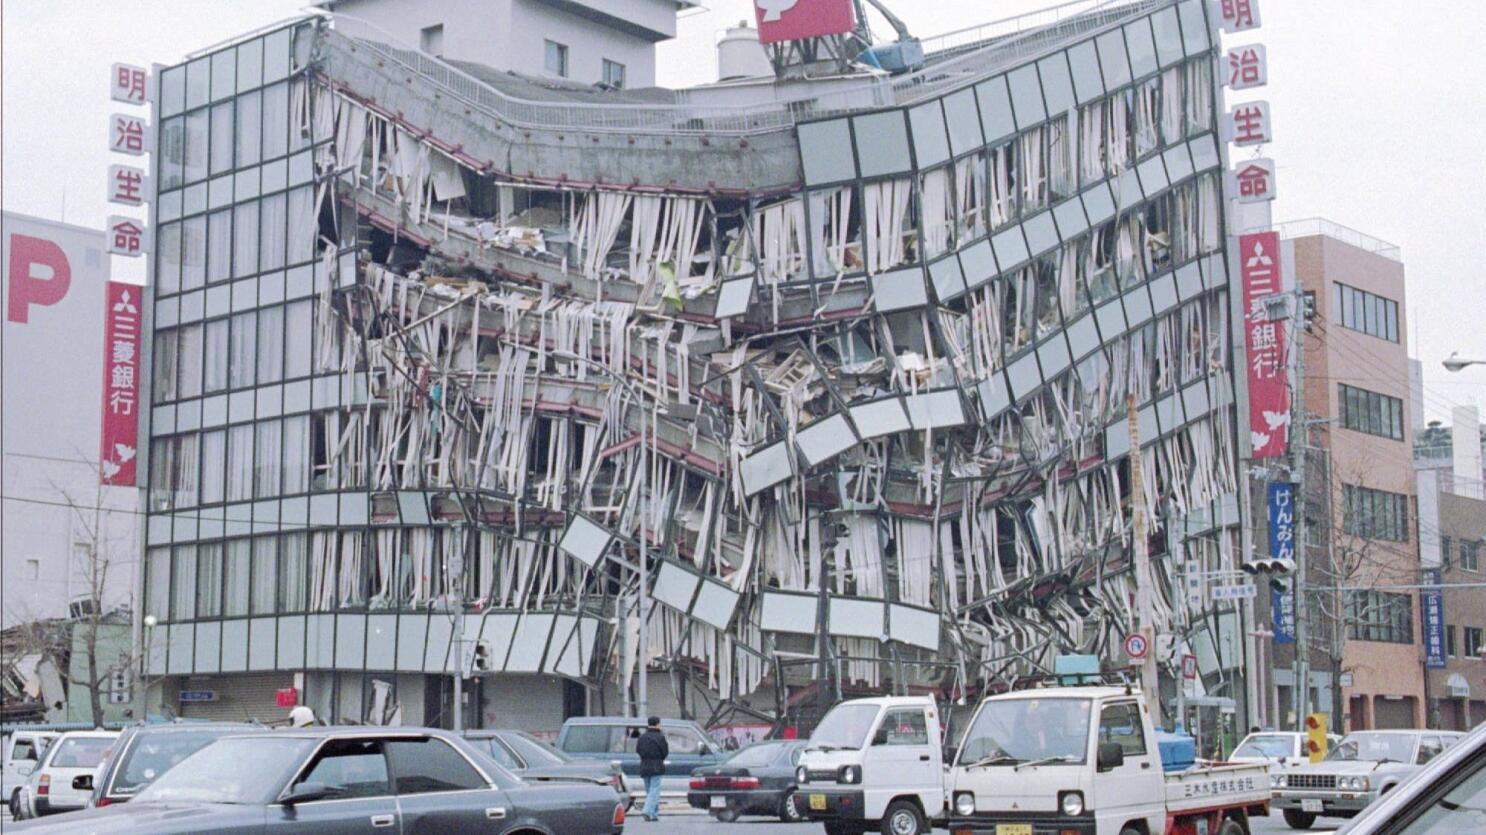
\includegraphics[width=1\linewidth]{Slike/screenshot004}
	\caption{Teško oštećena zgrada, potres Kobe, Japan 1995. god., Katsumi Kasahara / Novinar, Los Angeles Times }
	\label{fig:screenshot004_novo}
\end{figure}

\newpage

Potres Imperial Valley koji se desio 15. litropada 1979. godine bio je najveći potres u Kaliforniji tog desetljeća. Potres je bio magnitude 6,5 - te mu je epicentar bio u sjevernom Meksiku, a najviše štete na građevinama bilo je u gradu El Centro. Potres se osjetio od grada Las Vegas, pa sve do Tihog oceana. Zgrada Imperial County Service, koja se nalazi na slici 2.3,  jedna je od mnogih koje su nastradale u potresu. Najveći problem armirano-betonske zgrade bili su stupovi koji su se nalazili na istočnoj strani zgrade. Svi stupovi u redu popustili su, te je prvi kat zgrade pao za čak 30 cm [Slika 2.4]. 

\begin{figure}[h]
	\centering
	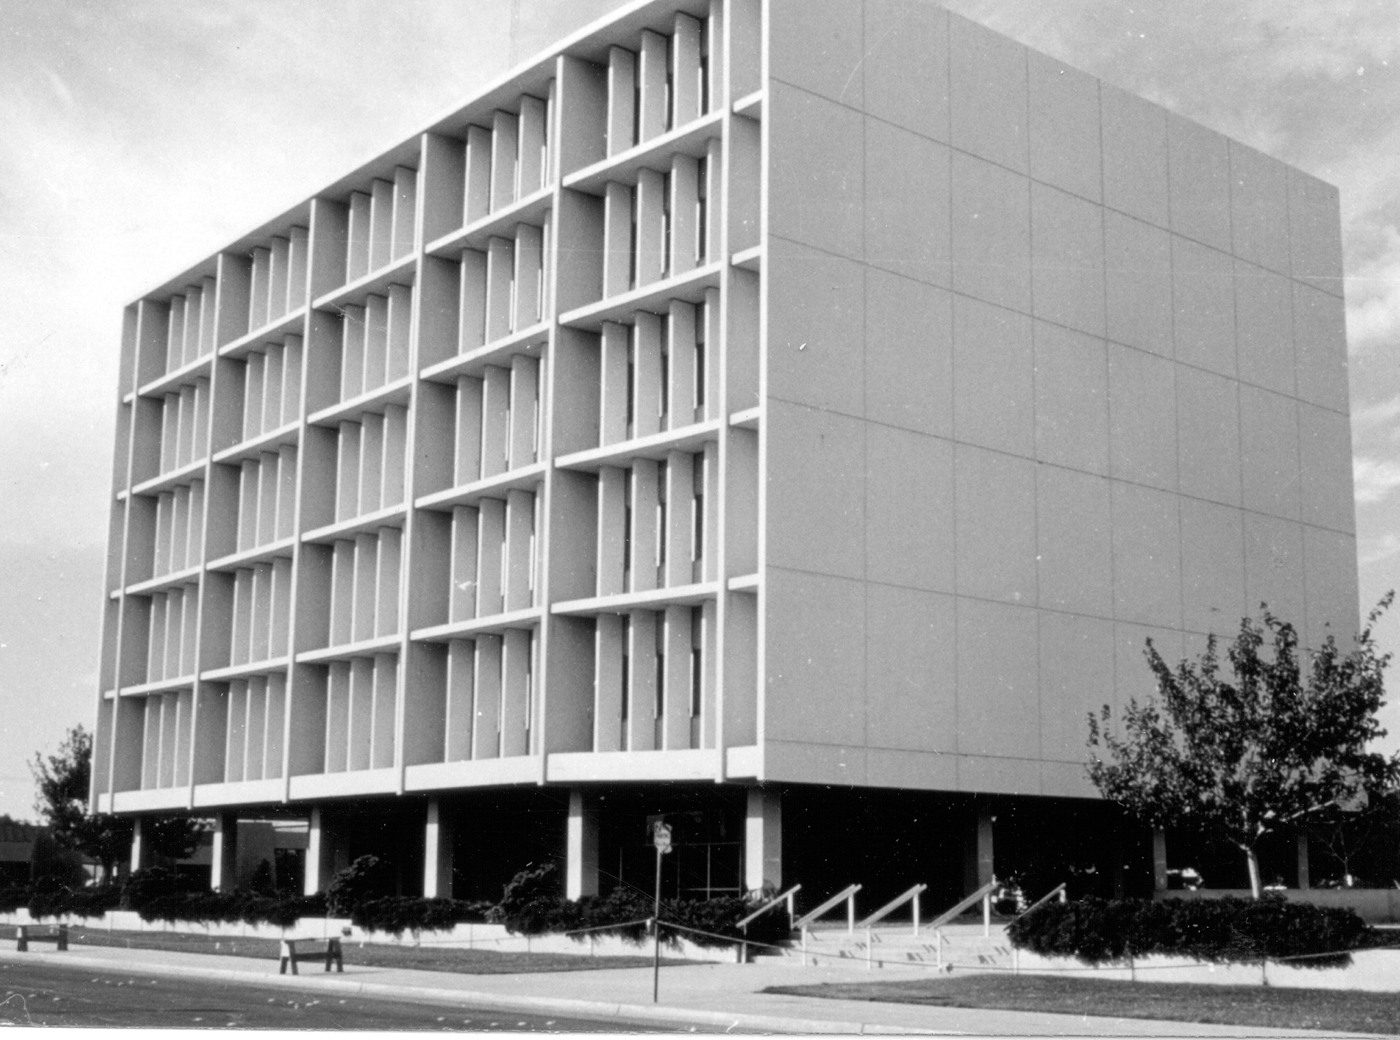
\includegraphics[width=1\linewidth]{Slike/imperial_valley}
	\caption{Zgrada Imperial County Service, El Centro, Kalifornia 1979. god., REPORT}
	\label{fig:imperialvalley}
\end{figure}

\begin{figure}[h]
	\centering
	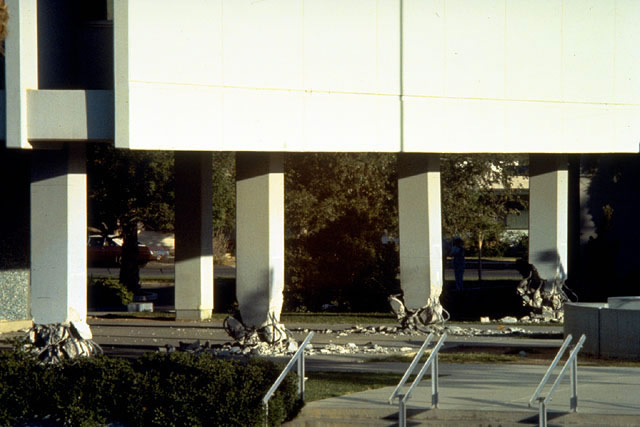
\includegraphics[width=1\linewidth]{Slike/imperial_valley_szupovi}
	\caption{Popušteni stupovi na zgradi Imperial County Service, El Centro, Kalifornia 1979. god., autor nepoznat}
	\label{fig:imperialvalleyszupovi}
\end{figure}

\newpage

Serija potresa u Cape Mandocinu desila se 25. travnja 1992. godine. Cape Mandecino zadesila su čak tri uzastopna potresa. Prvi i najjači bio je magnitude 7,2 - dok su sljedeća dva potresa bila magnitude 6,5. Sreća je bila da Cape Mandocino nije naseljeno područje, najveća šteta bila je u gradu Fernadel koji je udaljen odo 30 kilometara od epicentra. Nažalost u gradu bilo je oštećeno 32 građevine, od kojih je jedna Viktorijnska kuća [Slika 2.5] koja se pomakla i dimnjak se razdvojio od kuće, prije se dimnjak nalazio na mjestu gdje je siva crta.


\begin{figure}[h]
	\centering
	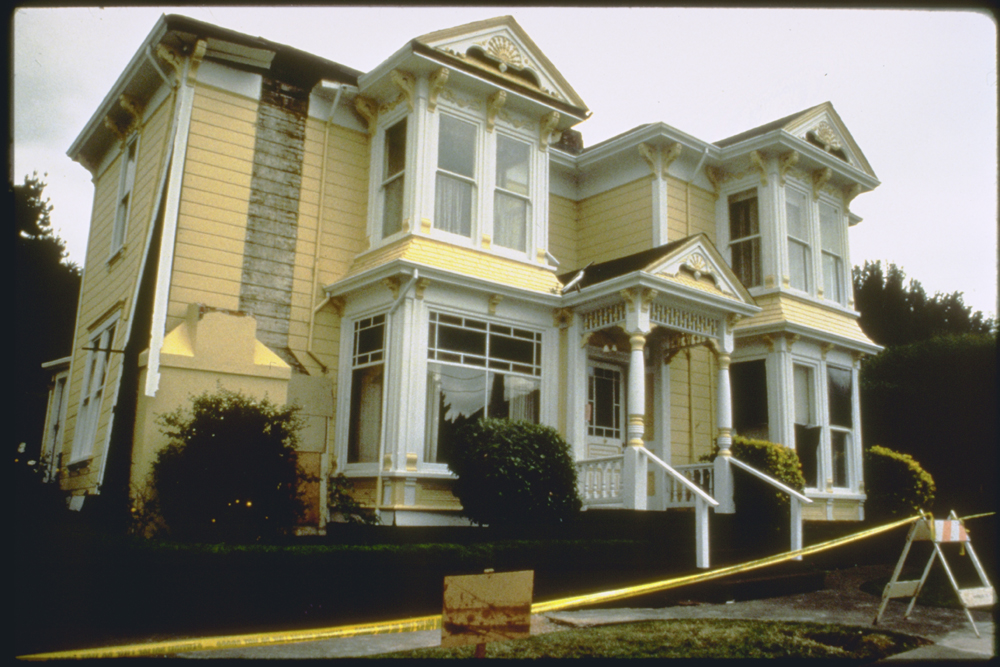
\includegraphics[width=1\linewidth]{Slike/cape_mandecino}
	\caption{Oštećena Viktorijanska kuća, Fernadel, Kalifornia, 1992. god., autor nepoznat, ONAJ ARTICLE }
	\label{fig:capemandecino}
\end{figure}


\chapter{JednadŽba kretanja}
U laboratorijskim ispitivanjima za bolje shvaćanje djelovanja potresa na konstrukcije koristi se jednokatni okvir na kojeg utječe pomicanje podloge (potres). Jednokatni okvir s krutom pločom koji mi promatramo ima samo jedan stupanj slobode, a to je horizontalni pomak ploče. Pošto nas zanima utjecaj promjene mase i širine ploče jednokatnog okvira na njegov dinamički odgovor, jedokatne okvire ćemo ispitivati samo na dinamičku pobudu podloge, bez nanošenja ostalih vanjskih sila. Sukladno tome jednadžbu kretanja dobit ćemo iz drugog Newtonovog zakona kojim ćemo izjednačiti dijagram slobodnog tijela (DST) s dijagramom masa puta akceleracija (DMA).


Na Slici 3.1 prikazana je skica jednokatnog okvira kojeg upotrebljavamo u pokusu, s lijeve strane okvir je u nedeformiranom stanju, a s desne strane on je u deformiranom stanju.

\begin{figure}[h]
	\centering
	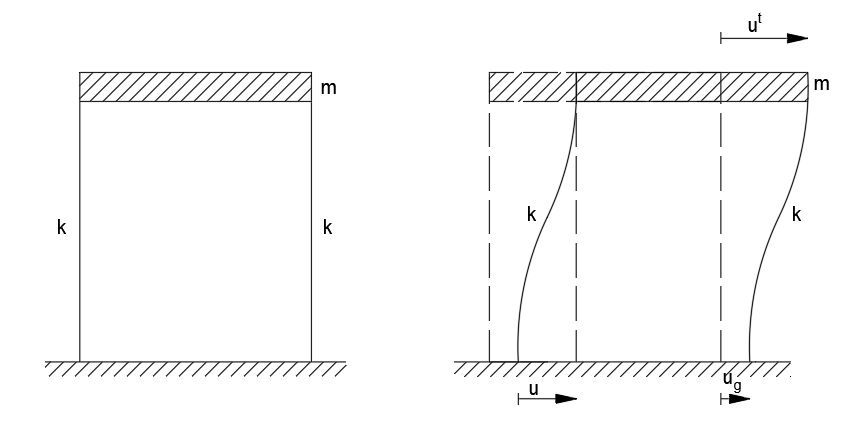
\includegraphics[width=1\linewidth]{Slike/screenshot003}
	\caption{Deformiranje jednokatnog okvira pri pobudi potresom}
	\label{fig:screenshot004}
\end{figure}


\newpage

Članovi na Slici 3.1 jesu:

m - masa,

k - krutost,

u - relativni pomak okvira,

$u^t$ - ukupni pomak,

$u_g$ - pomak tla (podloge).


\begin{figure}[h]
	\centering
	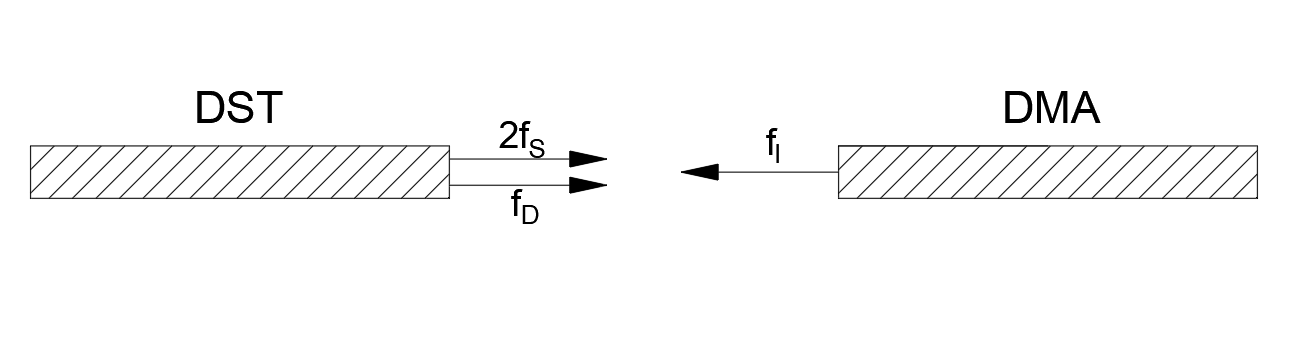
\includegraphics[width=1\linewidth]{Slike/screenshot002}
	\caption{DST i DMA dijagrami}
	\label{fig:screenshot002}
\end{figure}

Kada izjednačimo DST i DMA dijagram dobivamo:

\begin{equation}\label{Jednadžba 3.1}
	2f_S + f_D = - f_I,
\end{equation}

gdje su:

$2f_S$ - elastična sila od zidova jedokatnog okvira (NAPOMENA: U nastavku proračuna $2f_S$ biti će $f_S$ zbog toga što je krutost oba zida dana kao jedna vijednost prije početka pokusa.),

$f_D$ - sila prigušenja,

$f_I$ - sila inercije.

Elastična sila jednaka je:

\begin{equation}\label{Jednadzba 3.2}
	f_S = k*u.
\end{equation}

Sila prigušenja proporcionalna je brzini:

\begin{equation}\label{Jednadzba 3.3}
	f_D = c*\dot{u},
\end{equation}

a sila inercije jednaka je:

\begin{equation}\label{Jednadzba 3.4}
	f_I = m * \ddot{u^t},
\end{equation}

gdje su:

$c$ - koeficijent viskoznog prigušenja,

$\dot{u}$ - brzina,

$\ddot{u}$ - ubrzanje.

\newpage

Uvrštavanjem jednakosti sila, slijedi:

\begin{equation}\label{Jednadzba 3.5}
	k*u + c*\dot{u} = - m*\ddot{u}^t,
\end{equation}

odnosno:

\begin{equation}\label{Jednadzba 3.6}
	k*u + c*\dot{u} + m*\ddot{u}^t =0.
\end{equation}

Iz Slike (3.1) vidimo da je ukupni pomak $u^t$ jednak zbroju pomaka tla i relativnog pomaka okvira:

\begin{equation}\label{Jednadzba 3.7}
	u^t = u_g + u.
\end{equation}

Deriviranjem jednažbe (\ref{Jednadzba 3.7}) dobivamo:

\begin{equation}\label{Jednadzba 3.8}
	\dot{u^t} = \dot{u_g} + \dot{u},
\end{equation}

gdje su:

$\dot{u^t}$ - ukupna brzina,

$\dot{u_g}$ - brzina tla (podloge),

$\dot{u}$ - relativna brzina okvira,

te iz druge derivacije slijedi:

\begin{equation}\label{Jednadzba 3.9}
	\ddot{u^t} = \ddot{u_g} + \ddot{u},
\end{equation}

gdje su:

$\ddot{u^t}$ - ukupno ubrzanje,

$\ddot{u_g}$ - ubrzanje tla (podloge),

$\ddot{u}$ - relativno ubrzanje okvira.

Uvrštavanjem jednadžbe (\ref{Jednadzba 3.9}) u jednadžbu (\ref{Jednadzba 3.6}) dobivamo:

\begin{equation}\label{Jednadzba 3.10}
	k*u + c*\dot{u} + m*(\ddot{u_g} + \ddot{u}) = 0,
\end{equation}

odnosno:

\begin{equation}\label{Jednadzba 3.11}
	k*u + c*\dot{u} + m*\ddot{u} = - m*\ddot{u_g}.
\end{equation}

Preko ovih izraza dobili smo jednadžbu kretanja koja nam je potrebna za daljnji proračun.

Sve vrijednosti u jednadžbi smo ili odredili iz dimenzija konstrukcije (masa i krutost zidova), ili ćemo ih dobiti rezultatima mjerenja. Jedina nepoznanica nam je koeficijent viskoznog prigušenja za kojeg sljedi objašnjenje i izvod formule.

\newpage



Koeficijent viskoznog prigušenja jest:

\begin{equation}\label{Jednadzba 3.12}
	c = \zeta * \omega *2m,
\end{equation}

gdje su:

$\zeta$ - prigušenje

$\omega$ - kružna frekvencija.

Prigušenje ne možemo odrediti analitički, već ga određujemo iz rezultata koje dobivamo iz laboratorijskog ispitivanja slobodnih oscilacija okvira. Ono zapravo opisuje razliku između dvaju uzastopnih brijegova amplitude.

Stoga, izraz za prigušenje glasi:

\begin{equation}\label{Jednadzba 3.13}
	\zeta = \frac{1}{2\pi} * ln\frac{u_i}{u_{i+j}},
\end{equation}

gdje su:

$u_i$, $u_{i+j}$ - amplitude valova.

Kružna frekvencija:

\begin{equation}\label{Jednadzba 3.14}
	\omega = 2 * \pi * f
	[\frac{rad}{s}] 
\end{equation}

\begin{center}
	ili
\end{center}

\begin{equation}\label{Jednadzba 3.15}
	\omega = \sqrt{\frac{k}{m}},
\end{equation}

gdje je:

$f$ - vlastita frekvencija.

Vlastitu frekvenciju dobivamo kao:

\begin{equation}\label{Jednadzba 3.16}
	f = \frac{1}{T} [Hz],
\end{equation}

gdje je:

$T$ - period.

Period T možemo dobiti iz razlike dvaju susjednih brijegova amplitude iz rezultata ispitivanja slobodnih oscilacija ili uvrštavanjem jednažbe (\ref{Jednadzba 3.16}) u jednadžbu (\ref{Jednadzba 3.14}), te dobivamo:

\begin{equation}\label{Jednadzba 3.17}
	T = \frac{2\pi}{\omega}.
\end{equation}



\chapter{Opis opreme i jednokatnog okvira}

\section{Laboratorijska oprema}

\subsection{Opti\v cki mjerni sustav GOM mbH PONTOS 3D 4M}

Optički mjerni sustav sastoji se od mjerne glave s dvije kamere, kablova, nosača, kalibracijskog objekta, para leća, laserskog pokazivača, kofera, LED osvjetljenja, foto ćelija.

Sustav kamera koristi se za 3D beskontaktno optičko mjerenje pomaka i deformacija. Prije početka snimanja pokusa, potrebno je napraviti kalibraciju kamera, odnosno ovisno o veličini objekta koji se snima potrebno ih je namjestiti na određenu udaljenost i kut snimanja. Kamere snimaju cijeli tijek pokusa. Na temelju praćenja objekta koje snimaju, u našem slučaju jednokatnog okvira, kao rezultat daju podatke o položaju točaka na površini jednokatnog okvira. Točke koje se prate su zapravo crno-bijele referentne točke koje se lijepe na povšinu jednokatnog okvira i podloge kako bi ih kamere mogle pratiti u svim fotografijama koje one snime. Obzirom na to da na model stavljamo referentne točke, prva fotografija u nizu naziva se referentna fotografija, a nakon nje sljedi niz fotografija kojima određujemo rezultate mjerenja.
\vspace{1cm}

Tehničke karakteristike:

- mogućnost snimanja do 168 fps rezolucijom od 2400 x 1728 piksela, te do 1300 fps rezolucijom od 2400 x 168 piksela,

- jedan par leća žarišne dužine 20 mm pogodan za mjerne volumene od 125 x 90 $mm^2$ do 2150 x 1600 $mm^2$,

- kalibracijski objekt za snimanje mjernog volumena od 350 x 260 $m^2$ do 500 x 370 $mm^2$.

\begin{figure}[h]
	\centering
	%\includegraphics[width=0.7\linewidth]{"C:/Users/Lovro Korpar/AppData/Local/Packages/5319275A.WhatsAppDesktop_cv1g1gvanyjgm/TempState/D43EC839A158DC7EFA4CF0520781925B/WhatsApp Image 2023-08-23 at 13.03.57"}
	\caption{Optički mjerni sustav GOM mbH PONTOS 3D 4M, slikano u laboratoriju za konstrukcije}
	\label{fig:whatsapp-image-2023-08-23-at-13}
\end{figure}

\newpage

\subsection{Sustav od dvije dvoosne potresne platforme Quanser STI-III}

Sustav od dvije dvoosne potresne platforme Quanser STI-III pokretane elektromagnetskim motorom. Sustav se sastoji od kontrolne \textit{hardware} ploče sa potrebnim \textit{software-om}, te od podložne ploče za dvoosne platforme.

Sustav služi za modelska ispitivanja na utjecaj dinamičke pobude. Dvije platforme se mogu koristiti odvojeno i neovisne su jedna o drugoj. Moguće je izvoditi dva ispitivanja istovremeno, ali i zajedno na način da model bude oslonjen na obje platforme. Pri korištenju platformi istovremeno dopuštena je veća maksimalna masa, a pobuda koju one proizvode može biti jednaka (sinkroni rad) ili različita (asinkroni rad). CITIRANO IZ POPISA OPREME

\newpage

Tehničke karakteristike:

- tlocrtne dimenzije svake platforme 625 x 625 $mm^2$,

- hod svake platforme u svakom od dva smjera je 15 cm, a raspon radnih frekvencija između 0 i 20 Hz,

- svaka platforma uz maksimalni teret od 130 kg može proizvesti ubrzanje od 1g u svakom od dva smjera,

- svaka platforma bez ikakvog tereta može proizvesti ubrzanje od 2,8g u x smjeru i 4,5g u y smjeru,

- osna udaljenost platformi može biti od 1 m do 2,5 m.

SLIKA

\section{Jednokatni okvir}

Za izvedbu laboratorijskih ispitivanja korišten je jednokatni okvir. On se sastoje od dvije krute ploče, dvije metalne ploče (zidovi), vijaka, te podložnih pločica koje se nalaze između krutih i metalnih ploča [Slika 4.2].

Ukupna masa okvira iznosi 1483 grama, no s obzirom da je donja kruta ploča povezana sa potresnom platformom nju možemo zanimariti, isto kao i ostatak donje polovice okvira na kojoj nema učinka pri oscilaciji. Kada te stvari uzmemo u obzir ukupna masa okvira koja nam je potrebna za daljnji proračun iznosi 741,5 grama. 

S obzirom da sa laboratorijskim ispitivanjima želimo saznati kako promjena mase okvira utječe na dinamičku pobudu, drugom okviru dodali smo dva utega od kojih svaki ima težinu 1 N, tj. 101,97 grama. Znači ukupna masa drugog okvira iznosi 945,44 grama.

\begin{figure}[H]
	\centering
	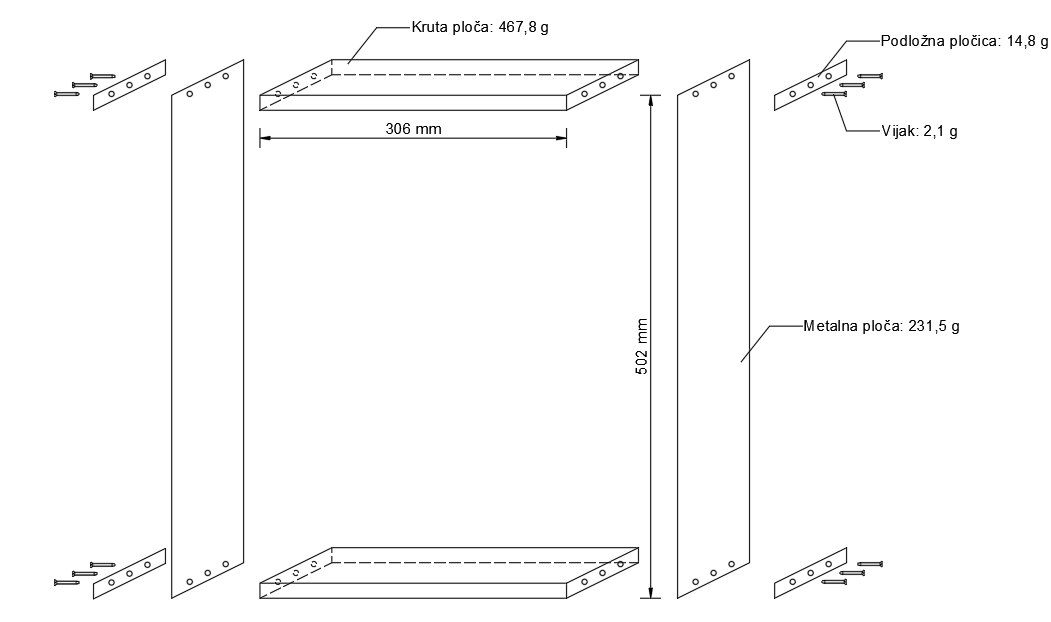
\includegraphics[width=1\linewidth]{Slike/okvir_skica}
	\caption{Skica jednokatnog okvira}
	\label{fig:okvirskica}
\end{figure}

KAKO NUMERIRATI TABLICE (NISU U POPISU TABLICA) I SLIKE NE IDU PO REDU (NE ZNAM ZASTO NE FUNKCIONIRA h)

\begin{table}[H]
	\label{table1}
	\caption{Opis tablice 1}
	\begin{center}
		\begin{tabular}{|l|c|c|r|}
			\hline
			Element & Komad & Masa[g] & Ukupna masa [g]\\
			\hline
			Kruta ploča & 2 & 467,8 & 935,6\\
			\hline
			Metalna ploča & 2 & 231,5 & 463\\
			\hline
			Podložna pločica & 4 & 14,8 & 59,2 \\
			\hline
			Vijak & 12 & 2,1 & 25,2\\
			\hline
			\multicolumn{3}{|l|}{Ukupna masa okvira} & 1483\\
			\hline
			\multicolumn{3}{|l|}{Ukupna masa gornjeg dijela okvira} & 741,5\\
			\hline
		\end{tabular}
	\end{center}
\end{table}


\begin{table}[H]
	\begin{center}
		\begin{tabular}{|l|c|c|r|}
			\hline
			Element & Komad & Masa[g] & Ukupna masa [g]\\
			\hline
			Kruta ploča & 2 & 467,8 & 935,6\\
			\hline
			Metalna ploča & 2 & 231,5 & 463\\
			\hline
			Podložna pločica & 4 & 14,8 & 59,2 \\
			\hline
			Vijak & 12 & 2,1 & 25,2\\
			\hline
			Uteg & 2 & 101,97 & 203,94\\
			\hline
			\multicolumn{3}{|l|}{Ukupna masa okvira} & 1686,94\\
			\hline
			\multicolumn{3}{|l|}{Ukupna masa gornjeg dijela okvira} & 945,44\\
			\hline
		\end{tabular}
	\end{center}
\end{table}

Prilikom izvođenja laboratorijskih ispitivanja korištena su dva jednokatna okvira [Slika 4.3]. Okvire smo istovremeno ispitivali na istoj potresnoj platformi kako bismo vidjeli odgovore jednokatnih okvira na istu pobudu izazvanu na potresnoj platformi. Okvire smo ispitivali istovremeno kako bi dobili točnije rezultate ispitivanja, ako bi ih ispitivali odvojeno ne bismo dobili istu pobudu podloge.


\begin{figure}[h]
	\centering
	%\includegraphics[width=1\linewidth]{"C:/Users/Lovro Korpar/AppData/Local/Packages/5319275A.WhatsAppDesktop_cv1g1gvanyjgm/TempState/66376C393BA5FAA7B07D3D4A0C7E3D02/WhatsApp Image 2023-09-06 at 18.52.48"}
	\caption{jednokatni okviri na potresnom stolu, gledano s desna na lijevo; okvir 1, okvir 2}
	\label{fig:whatsapp-image-2023-09-06-at-18}
\end{figure}

Okvir 1 [Slika 4.3] je bez dodane mase, njega ćemo usporediti sa okvirom 2 na kojem je dodana masa od 2 N [Slika 4.3], te ćemo vidjeti kako promjena mase utječe na dinamički odgovor na pobudu podloge.

\chapter{Laboratorijska ispitivanja i njihvi rezultati}

Laboratorijska ispitivanja provodili smo na Građevinskom fakultetu Sveučilišua u Rijeci u laboratoriju za konstrukcije. Za ispitivanja smo koristili potresnu platformu (opisano u poglavlju 4.1.2), optički mjerni sustav GOM (opisano u poglavlju 4.1.1), te dva jednokatna okvira (opisano u poglavlju 4.2), a za obradu optičkih podataka koristio se program ARAMIS professional.

Ukupno je provedeno pet laboratorijskih ispitivanja. Koristila su se dva jednokatna okvira koji su se ispitivali istovremeno [Slika 4.3]. Za oba okvira nanosile su se iste oscilacije podloge. 

U prvom ispitivanju promatrali smo slobodne oscilacije okvira. Potresni stol bio je u stanju mirovanja, a okvire smo pomakli rukom, te simulirali slobodne oscilacije. U drugom ispitivanju koristili smo se potresnim zapisom Northbridge. Za treće ispitivanje koristi smo potresni zapis Kobe, u četvrtom ispitivanju potresni zapis El Centro, a za peto ispitivanje koristili smo potresni zapis Cape Mandocio. Informacije o ovim potresnima opisane su u poglavlju 2.5.

\section{Rezultati ispitivanja}

\section{Ispitivanje slobodnih oscilacija}

\subsection{Okvir bez dodane mase}

Uz dobivenu krutost zidova koja iznosi 541,3 N/m i mase (TABLICA) možemo izračunati kružnu frekvenciju $\omega$, period $T$, te vlastitu frekvenciju $f$.

Uvrštavanjem krutosti i mase u jednadžbu (\ref{Jednadzba 3.15}) kružna frekvencija iznosi:

\begin{equation}
	\omega = \sqrt{\frac{541,3}{0,7415}} = 27,02 rad/s.
\end{equation}

Zatim uvrštavanjem kružne frekvencije u jednadžbu (\ref{Jednadzba 3.17}) dobivamo period $T$:

\begin{equation}
	T = \frac{2\pi}{27,02} = 0,23 s.
\end{equation}

A vlastitu frekvenciju dobivamo uvrštavanjem perioda $T$ u jednadžbu (\ref{Jednadzba 3.16}):

\begin{equation}
	f = \frac{1}{0,23} = 4,35 s^{-1}.
\end{equation}
%\cite{oluic2015}

\cite{chopra2007}





\cleardoublepage\phantomsection

%\printbibliography
\vspace{\baselineskip}
%\label{Bibliography}
\renewcommand{\bibname}{\uppercase{Literatura}}
\addcontentsline{toc}{chapter}{\textbf{Literatura}}
\bibliographystyle{unsrtnat-GFRI}

\bibliography{literatura1}
\bibliographystyle{vancouver}

\end{document}